\documentclass[11pt]{article}
\usepackage[margin=18mm,headheight=22pt]{geometry}
\usepackage{amsmath}
\usepackage{fontspec}
\usepackage{unicode-math}
\setmainfont{NewCM10}[Extension=.otf,UprightFont=*-Book,BoldFont=*-Bold,ItalicFont=*-BookItalic,BoldItalicFont=*-BoldItalic]
\setsansfont{NewCMSans10}[Extension=.otf,UprightFont=*-Book,BoldFont=*-Bold,ItalicFont=*-BookOblique,BoldItalicFont=*-BoldOblique]
\setmathfont{NewCMMath-Book.otf}
\usepackage{xcolor}
\definecolor{FAUblue}{HTML}{04316A}
\definecolor{Paperblue}{HTML}{EEF2F7}
\definecolor{EEIgold}{HTML}{CC9C42}
\usepackage{etoolbox,enumitem,booktabs,tabularx,array,needspace,microtype}
\usepackage[most]{tcolorbox}
\usepackage{titlesec,fancyhdr}
\usepackage[hidelinks]{hyperref}
\usepackage{draftwatermark}
\SetWatermarkText{Made by Thanate Amornjiraporn (Focus)}
\SetWatermarkColor{black!7}\SetWatermarkFontSize{30pt}\SetWatermarkAngle{45}
\setlength{\parindent}{0pt}
\setlength{\parskip}{5pt}
\setlist{itemsep=2pt,topsep=3pt,leftmargin=1.6em,beginpenalty=10000,endpenalty=10000}
\raggedbottom
\clubpenalty=10000 \widowpenalty=10000 \displaywidowpenalty=10000 \interlinepenalty=10000
\setcounter{secnumdepth}{0}
\setcounter{tocdepth}{1}
\pagestyle{fancy}\fancyhf{}
\fancyhead[L]{\small\sffamily\color{FAUblue} From Fundamentals to AI Apocalypse · APDR · Chapter 5}
\fancyhead[R]{\small\sffamily Memory Organisation}
\fancyfoot[C]{\small\thepage}
\titleformat{\section}{\Large\bfseries\sffamily\color{FAUblue}}{}{0pt}{}
\titleformat{\subsection}{\large\bfseries\sffamily\color{FAUblue}}{}{0pt}{}
\titlespacing*{\section}{0pt}{16pt}{6pt}
\preto\section{\Needspace{8\baselineskip}}
\preto\subsection{\Needspace{6\baselineskip}}
\newtcolorbox{equationcard}[1]{colback=Paperblue,colframe=Paperblue,boxrule=0pt,arc=0pt,left=10pt,right=10pt,top=6pt,bottom=6pt,title={#1},fonttitle=\small\bfseries\sffamily,coltitle=FAUblue,before skip=8pt,after skip=8pt}
\newtcolorbox{workedbox}[1]{colback=white,colframe=EEIgold,boxrule=0pt,leftrule=3pt,arc=0pt,left=10pt,top=4pt,bottom=4pt,title={#1},fonttitle=\small\bfseries\sffamily,coltitle=FAUblue,attach title to upper={\par},before skip=8pt,after skip=8pt}
\newtcolorbox{recallbox}[1]{colback=white,colframe=FAUblue,boxrule=0pt,leftrule=3pt,arc=0pt,left=10pt,top=4pt,bottom=4pt,title={#1},fonttitle=\small\bfseries\sffamily,coltitle=FAUblue,attach title to upper={\par},before skip=8pt,after skip=8pt}
\usepackage{environ}
\newsavebox\measurebox
% Typeset the section once invisibly to measure it; start a new page if it will not fit in what is left.
\makeatletter
\newif\ifkeep@measuring
\NewEnviron{keepsection}{%
  \ifkeep@measuring \BODY \else
    \edef\keep@sec{\the\value{section}}\edef\keep@sub{\the\value{subsection}}%
    \setbox\measurebox\vbox{\hsize\linewidth\keep@measuringtrue\def\Needspace##1{}\BODY}%
    \setcounter{section}{\keep@sec}\setcounter{subsection}{\keep@sub}%
    \dimen2=\ht\measurebox \advance\dimen2\dp\measurebox
    \dimen@=\textheight
    \ifdim\pagegoal<\maxdimen
      \dimen@=\pagegoal \advance\dimen@-\pagetotal
      \ifdim\dimen2>\dimen@ \clearpage \dimen@=\textheight \fi
    \fi
    % if it fits, nothing inside may force an early break
    \ifdim\dimen2>\dimen@ \BODY \else \begingroup\def\Needspace##1{}\BODY\endgroup \fi
  \fi}
\makeatother
\newtcolorbox{notebox}{colback=Paperblue,colframe=Paperblue,boxrule=0pt,arc=0pt,left=8pt,right=8pt,top=4pt,bottom=4pt,before skip=6pt,after skip=6pt}
\newtcolorbox{plainbox}{colback=white,colframe=FAUblue,boxrule=0pt,leftrule=3pt,arc=0pt,left=10pt,right=8pt,top=4pt,bottom=4pt,before skip=6pt,after skip=8pt}
\usetikzlibrary{arrows.meta}
\title{\sffamily\bfseries\color{FAUblue}Memory Organisation}
\author{Algorithms, Programming, and Data Representation \ensuremath{\cdot} Module 92313 \ensuremath{\cdot} Chapter 5\\[2pt]\small From Fundamentals to AI Apocalypse · personal study guide}
\date{}
\begin{document}
\maketitle
\begingroup\footnotesize\setlength{\parskip}{0pt}\tableofcontents\endgroup
\clearpage

\Needspace{8\baselineskip}
{\large This chapter explains how computers organise memory, identify locations, lay out multi-byte values, assemble memory modules, and distribute addresses across modules.}


\begin{keepsection}
\Needspace{13\baselineskip}
\section{Start from memory}

\Needspace{10\baselineskip}
Try each question first. Mark it sure, unsure, or guessed.

\Needspace{8\baselineskip}
\begin{enumerate}
\item Which is faster: CPU registers, RAM, or a hard disk?
\item What does a byte address select?
\item Which byte goes first in little-endian order?
\item How many bits select one of four memory modules?
\item What is the difference between high-order and low-order interleaving?
\end{enumerate}

\nopagebreak[4]{\small\itshape Answers: see “Start from memory” under Answers at the end.}
\end{keepsection}

\begin{keepsection}
\Needspace{17\baselineskip}
\section{How to use this guide}

\Needspace{14\baselineskip}
Study a section, hide it, then rebuild its rules and examples from memory. Attempt mixed practice before opening answers.

\Needspace{11\baselineskip}
\begin{enumerate}
\item \textbf{Day 0:} Try the cold start and study §5.1–5.2; solve practice 1, 4, 6, 21.
\item \textbf{Day 1:} Reconstruct byte-order rules in §5.3; solve practice 2, 7, 12, 19.
\item \textbf{Day 3:} Work through chip sizing in §5.4; solve practice 3, 8, 11, 13, 17.
\item \textbf{About day 7:} Rebuild both interleaving schemes in §5.5; solve practice 5, 10, 14, 18.
\item \textbf{About day 14:} Complete both exam problems without notes; explain each answer aloud.
\item \textbf{Before the exam:} Tick only skills you can demonstrate cold; revisit sections named in missed answers.
\end{enumerate}

\begin{notebox}\textbf{When stuck:} write the address width, addressable unit, row width, and byte order before calculating. Check units at the end.\end{notebox}
\end{keepsection}

\begin{keepsection}
\Needspace{16\baselineskip}
\section{How the chapter fits together}

\Needspace{13\baselineskip}
Memory properties motivate a hierarchy. Addresses select locations, byte order explains multi-byte layout, chips build capacity and width, and interleaving distributes requests.

\Needspace{8\baselineskip}
\textbf{Measure} \ensuremath{\cdot} capacity and access

\Needspace{6\baselineskip}
\begin{itemize}
\item 
\Needspace{4\baselineskip}
\textbf{Memory hierarchy} \hfill{\small\color{FAUblue}§5.1}

\Needspace{4\baselineskip}
speed \ensuremath{\cdot} cost \ensuremath{\cdot} capacity \ensuremath{\cdot} volatility

Rests on: identifying what each memory level trades away.

\item 
\Needspace{4\baselineskip}
\textbf{Addressing and capacity} \hfill{\small\color{FAUblue}§5.2}

\Needspace{4\baselineskip}
locations = 2\textsuperscript{address bits}

Rests on: the addressable unit and memory row width.

\end{itemize}

\Needspace{7\baselineskip}
\textbf{Define} \ensuremath{\cdot} interpret layout

\Needspace{5\baselineskip}
\begin{itemize}
\item 
\Needspace{4\baselineskip}
\textbf{Byte ordering} \hfill{\small\color{FAUblue}§5.3}

\Needspace{4\baselineskip}
MSB first / LSB first

Rests on: addresses identifying successive bytes of one value.

\item 
\Needspace{4\baselineskip}
\textbf{Chips and modules} \hfill{\small\color{FAUblue}§5.4}

\Needspace{4\baselineskip}
rows \ensuremath{\times} width

Rests on: multiplying row count by bits per row.

\end{itemize}

\Needspace{5\baselineskip}
\textbf{Derive} \ensuremath{\cdot} select and distribute

\Needspace{3\baselineskip}
\begin{itemize}
\item 
\Needspace{4\baselineskip}
\textbf{Interleaving} \hfill{\small\color{FAUblue}§5.5}

\Needspace{4\baselineskip}
address = module bits + row bits

Rests on: separating module selection from row selection.

\end{itemize}

\Needspace{10\baselineskip}
\Needspace{10\baselineskip}
\begin{center}\small\begin{tabularx}{\linewidth}{>{\raggedright\arraybackslash}X>{\raggedright\arraybackslash}X}\toprule
\textbf{Question} & \textbf{Method} \\ \midrule
How much memory? & Count addresses or multiply rows by width. \\
What byte appears first? & Identify endian convention, then order bytes. \\
Where does this address go? & Split module-selection and row bits. \\
\bottomrule\end{tabularx}\end{center}
\end{keepsection}

\begin{keepsection}
\Needspace{11\baselineskip}
\section{5.1 Memory hierarchy and properties}

\Needspace{8\baselineskip}
Hierarchy balances speed, capacity, cost, volatility, and flexibility. Registers are fastest and smallest; storage devices are largest and slowest.

\Needspace{12\baselineskip}
\begin{plainbox}\textbf{In plain words:} memory is a ladder of trade-offs: the faster a memory is, the smaller and more expensive it is. Registers inside the processor are fastest; RAM is larger and slower; disks and SSDs are largest and slowest but keep their contents without power. SRAM and DRAM are two ways to build RAM: SRAM is faster, DRAM denser and cheaper.\end{plainbox}

\begin{equationcard}{Memory hierarchy}
\[ \begin{gathered} \text{fastest}/\text{smallest}\, \to \, \text{registers}\, \to \, \text{RAM}\, \to \, \text{storage}\, \to \, \text{largest}/\text{slowest} \end{gathered} \]
{\small \emph{Read it as: “from fastest and smallest to largest and slowest: registers, then RAM, then storage”.}\par This is a qualitative ordering, not a universal timing specification.}
\end{equationcard}

\Needspace{14\baselineskip}
\begin{center}
\begin{minipage}[t]{0.950\linewidth}\centering
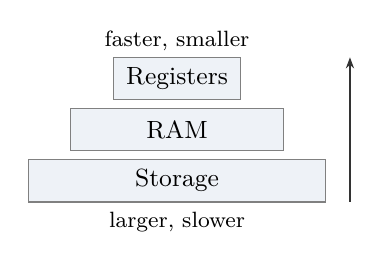
\begin{tikzpicture}
\node[,inner sep=1pt,font=\footnotesize] at (2.340,-0.216) {faster, smaller};
\filldraw[draw=black!50,fill=Paperblue] (1.530,-0.432) rectangle (3.150,-0.972);
\node[,inner sep=1pt,font=\small] at (2.340,-0.702) {Registers};
\filldraw[draw=black!50,fill=Paperblue] (0.990,-1.080) rectangle (3.690,-1.620);
\node[,inner sep=1pt,font=\small] at (2.340,-1.350) {RAM};
\filldraw[draw=black!50,fill=Paperblue] (0.450,-1.728) rectangle (4.230,-2.268);
\node[,inner sep=1pt,font=\small] at (2.340,-1.998) {Storage};
\draw[-{Stealth[length=4pt]},black!80] (4.536,-2.268) -- (4.536,-0.432);
\node[,inner sep=1pt,font=\footnotesize] at (2.340,-2.520) {larger, slower};
\end{tikzpicture}\par\smallskip{\small\raggedright \textbf{The memory hierarchy.} Each level down holds more and costs less per bit, but takes longer to reach.\par}\end{minipage}
\end{center}

Memory holds data, instructions, and addresses as binary values. Contents change only when overwritten. Registers are fixed in the CPU; RAM is expandable main memory; disks and other devices provide expandable storage. The lecture’s comparison is qualitative: registers are expensive, small, fast, volatile; RAM is intermediate; disks are cheap, large, slower, and non-volatile.

\begin{keepsection}
\Needspace{15\baselineskip}
\subsection{SRAM and DRAM}

\Needspace{12\baselineskip}
Static RAM (SRAM) is fast, less dense because each bit needs more transistors, and used mainly for cache; the slides also say it consumes less power. Dynamic RAM (DRAM) stores a bit in a transistor and capacitor. The capacitor leaks its charge, so DRAM must be refreshed periodically. It is cheaper but slower than SRAM and is used mainly for main memory.

\Needspace{10\baselineskip}
\begin{center}\small\begin{tabularx}{\linewidth}{>{\raggedright\arraybackslash}X>{\raggedright\arraybackslash}X>{\raggedright\arraybackslash}X}\toprule
\textbf{Type} & \textbf{Cell and behaviour} & \textbf{Main use in the lecture} \\ \midrule
SRAM & More transistors per bit; faster, less dense, lower power & Cache \\
DRAM & Transistor and capacitor; needs periodic refresh & Main memory \\
\bottomrule\end{tabularx}\end{center}

\begin{workedbox}{Worked example}
A program, its data, and pointers to both can all be represented as binary values.

\Needspace{2\baselineskip}
\begin{enumerate}
\item CPU instructions, data values, and addresses all use binary storage. \hfill{\small\color{FAUblue}§5.1}
\end{enumerate}
\end{workedbox}

\Needspace{5\baselineskip}
\begin{notebox}\textbf{Trap:} state the addressable unit, width, and byte order before calculating. Do not treat a qualitative lecture comparison as a fixed hardware specification.\end{notebox}

\Needspace{6\baselineskip}
\Needspace{6\baselineskip}
\begin{notebox}\textbf{Near miss:} DRAM holds data for as long as the computer runs, so it can seem permanent, but it is volatile: it needs power and constant refreshing, and switching off loses its contents, unlike flash storage.\end{notebox}

\Needspace{13\baselineskip}
\begin{recallbox}{Recall check \ensuremath{\cdot} answer without looking}
\Needspace{8\baselineskip}
\begin{enumerate}
\item Why can a computer use a small amount of fast memory together with much larger, slower storage?
\item Name three things memory can store.
\item Which RAM type is used mainly for cache, and which for main memory?
\item Why does DRAM need refreshing, and how does its speed compare with SRAM?
\end{enumerate}

\nopagebreak[4]{\small\itshape Answers: see “5.1 Memory hierarchy and properties” under Answers at the end.}
\end{recallbox}
\end{keepsection}
\end{keepsection}

\begin{keepsection}
\Needspace{9\baselineskip}
\section{5.2 RAM cells, addressing, and capacity}

\Needspace{6\baselineskip}
A memory needs a way to identify locations and a unit that each address selects.

\Needspace{10\baselineskip}
\begin{plainbox}\textbf{In plain words:} think of memory as a table of numbered rows. The \textbf{address} is the row number, and each row holds a fixed number of bits, the addressable unit (often one byte). With \textit{k} address bits you can number 2\textsuperscript{\textit{k}} rows, so the capacity is the number of rows times the bits per row.\end{plainbox}

\begin{equationcard}{Memory size}
\[ \begin{gathered} {R}\, \text{rows}\, \times \, {W}\, \text{bits}\, \text{per}\, \text{row}\, =\, {R}\times {W}\, \text{bits} \end{gathered} \]
{\small \emph{Read it as: “R rows times W bits per row is R \ensuremath{\times} W bits”.}\par Address count depends on address width and the addressable unit.}
\end{equationcard}

\Needspace{14\baselineskip}
\begin{center}
\begin{minipage}[t]{0.950\linewidth}\centering
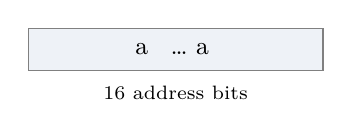
\begin{tikzpicture}
\filldraw[draw=black!50,fill=Paperblue] (0.072,-0.360) rectangle (3.816,-0.900);
\node[,inner sep=1pt,font=\small] at (1.944,-0.630) {a₁₅ … a₀};
\node[,inner sep=1pt,font=\scriptsize] at (1.944,-1.188) {16 address bits};
\end{tikzpicture}\par\smallskip{\small\raggedright \textbf{16 address bits} number 2\textsuperscript{16} = 65 536 rows: each extra bit doubles the count.\par}\end{minipage}
\end{center}

\Needspace{12\baselineskip}
RAM can be modelled as R rows of W bits: total capacity is R\ensuremath{\times}W bits. Byte-addressable memory assigns one address to each byte; word-addressable memory assigns one address to each processor word. For n address bits there are 2\textsuperscript{n} distinct addresses. If each address selects one byte, capacity is 2\textsuperscript{n} bytes. The slides use binary capacity units: 1 KB=2\textsuperscript{10} bytes, 1 MB=2\textsuperscript{20}, 1 GB=2\textsuperscript{30}, 1 TB=2\textsuperscript{40}.

\begin{workedbox}{Worked example}
The lecture’s 1GB example has 256M rows \ensuremath{\times} 32 bits = 8,192M bits = 1,024M bytes = 1 GiB (binary units).

\Needspace{2\baselineskip}
\begin{enumerate}
\item 256M rows times 4 bytes per row equals 1,024M bytes. \hfill{\small\color{FAUblue}§5.2}
\end{enumerate}
\end{workedbox}

\Needspace{6\baselineskip}
\begin{notebox}\textbf{Trap:} state the addressable unit, width, and byte order before calculating. Do not treat a qualitative lecture comparison as a fixed hardware specification.\end{notebox}

\Needspace{5\baselineskip}
\begin{notebox}\textbf{Near miss:} a 16-bit address looks as if it should give 16 rows, but it gives 2\textsuperscript{16} = 65 536 rows: each extra address bit doubles the count.\end{notebox}

\Needspace{10\baselineskip}
\begin{recallbox}{Recall check \ensuremath{\cdot} answer without looking}
\Needspace{4\baselineskip}
\begin{enumerate}
\item Why does byte addressing make the address increment by one byte?
\item A RAM has 256M rows, 32 bits per row. How many bytes is this?
\end{enumerate}

\nopagebreak[4]{\small\itshape Answers: see “5.2 RAM cells, addressing, and capacity” under Answers at the end.}
\end{recallbox}
\end{keepsection}

\begin{keepsection}
\Needspace{10\baselineskip}
\section{5.3 Endianness and aligned access}

\Needspace{7\baselineskip}
When a value spans multiple bytes, the byte order determines what appears at increasing addresses.

\Needspace{11\baselineskip}
\begin{plainbox}\textbf{In plain words:} a number wider than one byte is spread over several addresses, so the order of its bytes needs a rule. \textbf{Big-endian} puts the most significant byte first, at the lowest address, the way we write numbers; \textbf{little-endian} puts the least significant byte first.\end{plainbox}

\begin{equationcard}{Byte order}
\[ \begin{gathered} \text{Big}-\text{endian}:\, \text{MSB}\, \text{at}\, \text{lowest}\, \text{address}\, \cdot \, \text{Little}-\text{endian}:\, \text{LSB}\, \text{at}\, \text{lowest}\, \text{address} \end{gathered} \]
{\small \emph{Read it as: “big-endian: most significant byte at the lowest address; little-endian: least significant byte at the lowest address”.}\par The starting address is the address of the first byte of the item.}
\end{equationcard}

\Needspace{14\baselineskip}
\begin{center}
\begin{minipage}[t]{0.465\linewidth}\centering
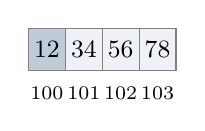
\begin{tikzpicture}
\filldraw[draw=black!50,fill=FAUblue!25] (0.072,-0.360) rectangle (0.540,-0.900);
\node[,inner sep=1pt,font=\small] at (0.306,-0.630) {12};
\node[,inner sep=1pt,font=\scriptsize] at (0.306,-1.188) {100};
\filldraw[draw=black!50,fill=Paperblue] (0.540,-0.360) rectangle (1.008,-0.900);
\node[,inner sep=1pt,font=\small] at (0.774,-0.630) {34};
\node[,inner sep=1pt,font=\scriptsize] at (0.774,-1.188) {101};
\filldraw[draw=black!50,fill=Paperblue] (1.008,-0.360) rectangle (1.476,-0.900);
\node[,inner sep=1pt,font=\small] at (1.242,-0.630) {56};
\node[,inner sep=1pt,font=\scriptsize] at (1.242,-1.188) {102};
\filldraw[draw=black!50,fill=Paperblue] (1.476,-0.360) rectangle (1.944,-0.900);
\node[,inner sep=1pt,font=\small] at (1.710,-0.630) {78};
\node[,inner sep=1pt,font=\scriptsize] at (1.710,-1.188) {103};
\end{tikzpicture}\par\smallskip{\small\raggedright \textbf{Big-endian}: 0x12345678 with its most significant byte, 12, at the lowest address.\par}\end{minipage}\hfill
\begin{minipage}[t]{0.465\linewidth}\centering
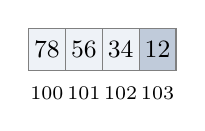
\begin{tikzpicture}
\filldraw[draw=black!50,fill=Paperblue] (0.072,-0.360) rectangle (0.540,-0.900);
\node[,inner sep=1pt,font=\small] at (0.306,-0.630) {78};
\node[,inner sep=1pt,font=\scriptsize] at (0.306,-1.188) {100};
\filldraw[draw=black!50,fill=Paperblue] (0.540,-0.360) rectangle (1.008,-0.900);
\node[,inner sep=1pt,font=\small] at (0.774,-0.630) {56};
\node[,inner sep=1pt,font=\scriptsize] at (0.774,-1.188) {101};
\filldraw[draw=black!50,fill=Paperblue] (1.008,-0.360) rectangle (1.476,-0.900);
\node[,inner sep=1pt,font=\small] at (1.242,-0.630) {34};
\node[,inner sep=1pt,font=\scriptsize] at (1.242,-1.188) {102};
\filldraw[draw=black!50,fill=FAUblue!25] (1.476,-0.360) rectangle (1.944,-0.900);
\node[,inner sep=1pt,font=\small] at (1.710,-0.630) {12};
\node[,inner sep=1pt,font=\scriptsize] at (1.710,-1.188) {103};
\end{tikzpicture}\par\smallskip{\small\raggedright \textbf{Little-endian}: the same value with its least significant byte, 78, at the lowest address.\par}\end{minipage}
\end{center}

\Needspace{13\baselineskip}
Big-endian stores the most significant byte first; little-endian stores the least significant byte first. Endianness changes the order of bytes in one multi-byte item, not the bit order inside each byte. A character string treated as individual ASCII bytes therefore retains its character order. Some architectures prohibit unaligned multi-byte accesses; the lecture identifies this as architecture-dependent.

\begin{workedbox}{Worked example}
A 16-bit value A9A1 beginning at byte address 2 is aligned in the slide’s example; F021 beginning at address 7 is unaligned.

\Needspace{3\baselineskip}
\begin{enumerate}
\item Determine alignment from the access width and starting address; the lecture’s examples contrast 2 with 7. \hfill{\small\color{FAUblue}§5.3}
\end{enumerate}
\end{workedbox}

\Needspace{7\baselineskip}
\begin{notebox}\textbf{Trap:} state the addressable unit, width, and byte order before calculating. Do not treat a qualitative lecture comparison as a fixed hardware specification.\end{notebox}

\Needspace{6\baselineskip}
\begin{notebox}\textbf{Near miss:} 0x12345678 stored little-endian from address 100 puts 0x78 at 100 and 0x12 at 103, so the bytes in address order read 78 56 34 12. That looks backwards, but it is the same value read with the other rule.\end{notebox}

\Needspace{9\baselineskip}
\begin{recallbox}{Recall check \ensuremath{\cdot} answer without looking}
\Needspace{4\baselineskip}
\begin{enumerate}
\item How would the bytes of 0x54BCFE30 appear from low to high addresses in each format?
\item Store the 16-bit value 0x0005 at address 24. What is at address 25 in each format?
\end{enumerate}

\nopagebreak[4]{\small\itshape Answers: see “5.3 Endianness and aligned access” under Answers at the end.}
\end{recallbox}
\end{keepsection}

\begin{keepsection}
\Needspace{10\baselineskip}
\section{5.4 Memory chips and modules}

\Needspace{7\baselineskip}
Chip organisation connects a chip’s row count and data width to the capacity and width of a module.

\Needspace{10\baselineskip}
\begin{plainbox}\textbf{In plain words:} a memory chip is a grid of rows, each a few bits wide. Larger memories combine chips: side by side to widen the data path, or added rows to hold more. A module’s capacity is simply the total of its chips’ bits.\end{plainbox}

\begin{equationcard}{Chip capacity}
\[ \begin{gathered} \text{rows}\, \times \, \text{bits}\, \text{per}\, \text{row}\, =\, \text{bits} \\ \text{divide}\, \text{by}\, 8\, \text{for}\, \text{bytes} \end{gathered} \]
{\small \emph{Read it as: “rows times bits per row gives bits; divide by 8 for bytes”.}\par Here M means 2\textsuperscript{20}, as in the lecture’s capacity convention.}
\end{equationcard}

\Needspace{14\baselineskip}
A chip described as 128M\ensuremath{\times}8 stores 128M rows of 8 bits, or 128 MB using the lecture’s binary convention. Chips can be combined in parallel to widen a module, and multiple banks/modules can build larger capacity. The slides show a 1GB (256M\ensuremath{\times}32-bit) memory assembled from alternative combinations of chips and modules.

\Needspace{10\baselineskip}
\begin{center}\small\begin{tabularx}{\linewidth}{>{\raggedright\arraybackslash}X>{\raggedright\arraybackslash}X>{\raggedright\arraybackslash}X>{\raggedright\arraybackslash}X}\toprule
\textbf{Modules} & \textbf{Chips in each module} & \textbf{Module capacity} & \textbf{Total} \\ \midrule
2 & 2 \ensuremath{\times} 128M\ensuremath{\times}16 & 512 MiB & 1 GiB \\
2 & 4 \ensuremath{\times} 128M\ensuremath{\times}8 & 512 MiB & 1 GiB \\
4 & 2 \ensuremath{\times} 64M\ensuremath{\times}16 & 256 MiB & 1 GiB \\
4 & 4 \ensuremath{\times} 64M\ensuremath{\times}8 & 256 MiB & 1 GiB \\
\bottomrule\end{tabularx}\end{center}

\begin{workedbox}{Worked example}
Four 128M\ensuremath{\times}8 chips provide 128M rows of 32 bits, or 512 MiB. Two such modules provide 1 GiB.

\Needspace{2\baselineskip}
\begin{enumerate}
\item Width combines in parallel; module capacity is rows times total width. \hfill{\small\color{FAUblue}§5.4}
\end{enumerate}
\end{workedbox}

\Needspace{6\baselineskip}
\begin{notebox}\textbf{Trap:} state the addressable unit, width, and byte order before calculating. Do not treat a qualitative lecture comparison as a fixed hardware specification.\end{notebox}

\Needspace{5\baselineskip}
\begin{notebox}\textbf{Near miss:} a 1M \ensuremath{\times} 4 chip looks like 4 MB, but it holds 1M rows of 4 bits, which is 4 Mbit = 512 KB, because a byte is 8 bits. Divide by 8 before writing bytes.\end{notebox}

\Needspace{9\baselineskip}
\begin{recallbox}{Recall check \ensuremath{\cdot} answer without looking}
\Needspace{4\baselineskip}
\begin{enumerate}
\item How can four 128M\ensuremath{\times}8 chips provide a 128M\ensuremath{\times}32-bit module?
\item How many 64M\ensuremath{\times}16 chips provide 256 MiB?
\end{enumerate}

\nopagebreak[4]{\small\itshape Answers: see “5.4 Memory chips and modules” under Answers at the end.}
\end{recallbox}
\end{keepsection}

\begin{keepsection}
\Needspace{13\baselineskip}
\section{5.5 Memory interleaving}

\Needspace{10\baselineskip}
Interleaving assigns addresses across modules so independent modules can serve requests in parallel.

\Needspace{14\baselineskip}
\begin{plainbox}\textbf{In plain words:} interleaving divides the addresses between several memory modules, and which address bits choose the module decides how. Take the module bits from the low end of the address (low-order interleaving) and consecutive addresses are dealt round the modules like cards round a table: while one module is still busy, the next address is already in another that can start straight away. Take them from the high end and each module holds one large block of consecutive addresses.\end{plainbox}

\begin{equationcard}{Address split for four modules}
\[ \begin{gathered} 22\, \text{address}\, \text{bits}\, =\, 2\, \text{module}\, \text{bits}\, +\, 20\, \text{row}\, \text{bits} \end{gathered} \]
{\small \emph{Read it as: “22 address bits are 2 bits that choose the module plus 20 bits that choose the row inside it”.}\par The 2 module bits select one of four modules; the 20 row bits select a row.}
\end{equationcard}

\Needspace{14\baselineskip}
\begin{center}
\begin{minipage}[t]{0.465\linewidth}\centering
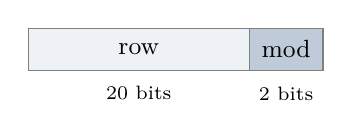
\begin{tikzpicture}
\filldraw[draw=black!50,fill=Paperblue] (0.072,-0.360) rectangle (2.880,-0.900);
\node[,inner sep=1pt,font=\small] at (1.476,-0.630) {row};
\node[,inner sep=1pt,font=\scriptsize] at (1.476,-1.188) {20 bits};
\filldraw[draw=black!50,fill=FAUblue!25] (2.880,-0.360) rectangle (3.816,-0.900);
\node[,inner sep=1pt,font=\small] at (3.348,-0.630) {mod};
\node[,inner sep=1pt,font=\scriptsize] at (3.348,-1.188) {2 bits};
\end{tikzpicture}\par\smallskip{\small\raggedright \textbf{Low-order interleaving}: the lowest 2 bits choose the module, so consecutive addresses go to different modules.\par}\end{minipage}\hfill
\begin{minipage}[t]{0.465\linewidth}\centering
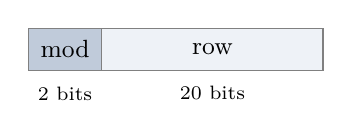
\begin{tikzpicture}
\filldraw[draw=black!50,fill=FAUblue!25] (0.072,-0.360) rectangle (1.008,-0.900);
\node[,inner sep=1pt,font=\small] at (0.540,-0.630) {mod};
\node[,inner sep=1pt,font=\scriptsize] at (0.540,-1.188) {2 bits};
\filldraw[draw=black!50,fill=Paperblue] (1.008,-0.360) rectangle (3.816,-0.900);
\node[,inner sep=1pt,font=\small] at (2.412,-0.630) {row};
\node[,inner sep=1pt,font=\scriptsize] at (2.412,-1.188) {20 bits};
\end{tikzpicture}\par\smallskip{\small\raggedright \textbf{High-order interleaving}: the top 2 bits choose the module, so each module holds one long run of addresses.\par}\end{minipage}
\end{center}

\Needspace{13\baselineskip}
The lecture’s example has 4M words, each 32 bits, built from four 1M\ensuremath{\times}32 modules. A 22-bit word address splits into 2 module bits and 20 row bits. High-order interleaving places module bits at the high end: consecutive addresses stay in one module for a large region. Low-order interleaving places module bits at the low end: consecutive addresses cycle across modules, supporting parallel access to adjacent data.

\begin{workedbox}{Worked example}
Low-order interleaving sends adjacent addresses to different modules; high-order interleaving groups a large contiguous range in one module.

\Needspace{2\baselineskip}
\begin{enumerate}
\item The address-bit positions determine whether nearby addresses are distributed or grouped. \hfill{\small\color{FAUblue}§5.5}
\end{enumerate}
\end{workedbox}

\Needspace{8\baselineskip}
\begin{notebox}\textbf{Trap:} state the addressable unit, width, and byte order before calculating. Do not treat a qualitative lecture comparison as a fixed hardware specification.\end{notebox}

\Needspace{7\baselineskip}
\begin{notebox}\textbf{Near miss:} high-order interleaving also splits memory across four modules, but with the module bits at the top of the address, a run of consecutive addresses stays inside one module, so reading them gets no parallel speed-up. For that, the module bits must come from the low end: low-order interleaving.\end{notebox}

\Needspace{9\baselineskip}
\begin{recallbox}{Recall check \ensuremath{\cdot} answer without looking}
\Needspace{4\baselineskip}
\begin{enumerate}
\item For low-order interleaving over four modules, where do addresses 8, 9, 10, and 11 go?
\item For high-order interleaving, which module contains addresses 0–3?
\end{enumerate}

\nopagebreak[4]{\small\itshape Answers: see “5.5 Memory interleaving” under Answers at the end.}
\end{recallbox}
\end{keepsection}

\begin{keepsection}
\Needspace{14\baselineskip}
\section{Formula map and units}

\Needspace{10\baselineskip}
\begin{center}\small\begin{tabularx}{\linewidth}{>{\raggedright\arraybackslash}X>{\raggedright\arraybackslash}X}\toprule
\textbf{Relation} & \textbf{Unit / meaning} \\ \midrule
Capacity = rows \ensuremath{\times} bits per row & bits; divide by 8 for bytes \\
n address bits \ensuremath{\to} 2\textsuperscript{n} addresses & locations \\
Byte-addressable capacity = 2\textsuperscript{n} bytes & bytes \\
Address bits = module bits + row bits & bits \\
1 KB=2\textsuperscript{10} bytes; 1 MB=2\textsuperscript{20}; 1 GB=2\textsuperscript{30}; 1 TB=2\textsuperscript{40} & binary units used in the lecture \\
\bottomrule\end{tabularx}\end{center}

\begin{notebox}\textbf{Check every answer:} distinguish bits from bytes; state the addressable unit; confirm the number of module and row bits sums to the address width.\end{notebox}
\end{keepsection}

\begin{keepsection}
\Needspace{10\baselineskip}
\section{Derive it cold}

\Needspace{7\baselineskip}
\begin{enumerate}
\item Derive the byte capacity of an R\ensuremath{\times}W-bit memory. \hfill{\small\color{FAUblue}§5.2}
\item Derive the maximum capacity of n-bit byte addressing. \hfill{\small\color{FAUblue}§5.2}
\item Derive module and row bit counts for four 1M\ensuremath{\times}32 modules. \hfill{\small\color{FAUblue}§5.5}
\item Derive the capacity of four parallel 128M\ensuremath{\times}8 chips. \hfill{\small\color{FAUblue}§5.4}
\end{enumerate}
\end{keepsection}

\begin{keepsection}
\Needspace{13\baselineskip}
\section{Explain it}

\Needspace{10\baselineskip}
\begin{enumerate}
\item Why are several memory types used instead of only the fastest one?
\item When does endianness affect the representation of a value?
\item Why do four 8-bit chips combine to make a 32-bit data path?
\item Why can low-order interleaving improve sequential access?
\item When does high-order interleaving fit the lecture’s use case?
\item Why must a capacity calculation state whether it counts bits or bytes?
\end{enumerate}

\nopagebreak[4]{\small\itshape Answers: see “Explain it” under Answers at the end.}
\end{keepsection}

\clearpage

\begin{keepsection}
\Needspace{10\baselineskip}
\section{Mixed practice}

\Needspace{7\baselineskip}
Try all 21 problems before showing the answers. The order mixes hierarchy, addressing, byte layout, chip sizing, and interleaving; choose the method yourself.

\begin{enumerate}
\item A four-bit address selects how many locations?
\item A 32-bit value is 54 BC FE 30. Give its byte order at increasing addresses in little-endian memory.
\item A 16M\ensuremath{\times}8 chip stores how many bytes?
\item Name two volatile memories from the lecture’s hierarchy.
\item For low-order interleaving across four modules, which module receives word address 15?
\item A 64-bit byte-addressed machine has how many byte addresses and what capacity do they represent?
\item Write the bytes of 0x0005 at addresses 24 and 25 in big-endian order.
\item How many 128M\ensuremath{\times}8 chips are needed for a 128M\ensuremath{\times}32 module?
\item Which is generally faster in the lecture’s hierarchy: registers or a hard disk?
\item For high-order interleaving with four modules, give module and row for address 2\textsuperscript{20}.
\item A memory has 2K rows of 16 bits. What is its capacity in bytes?
\item In big-endian storage, which byte is at the lowest address: MSB or LSB?
\item What is the capacity of a 64M\ensuremath{\times}8 chip?
\item Why can neighbouring instruction fetches benefit from low-order interleaving?
\item Does removing power preserve RAM contents according to the slides?
\item What capacity is represented by 2\textsuperscript{30} bytes using the lecture’s units?
\item What does 256M\ensuremath{\times}32 mean in the 1GB memory example?
\item For low-order interleaving, where do addresses 0, 1, 2, 3 go?
\item Does an ASCII string’s character order reverse in little-endian memory in the lecture example? Explain.
\item Which is larger: 1 TB or 1 GB, and by what factor under the lecture’s definitions?
\item Which statements distinguish SRAM from DRAM in the lecture?
\end{enumerate}

\nopagebreak[4]{\small\itshape Answers: see “Mixed practice” under Answers at the end.}
\end{keepsection}

\begin{keepsection}
\section{Exam-style problems}

\begin{keepsection}
\Needspace{13\baselineskip}
\subsection{1 \ensuremath{\cdot} Build and read a memory module \ensuremath{\cdot} 20 minutes}

\Needspace{10\baselineskip}
A system has 4M words of 32 bits, built from four 1M\ensuremath{\times}32 modules. It is byte-addressable and uses low-order interleaving.

\Needspace{7\baselineskip}
\begin{enumerate}
\item How many address bits are needed for all words?
\item How many module bits and row bits are used?
\item Which module and row receive word addresses 0 through 7?
\item Explain why sequential access may benefit.
\end{enumerate}

\nopagebreak[4]{\small\itshape Answers: see “Exam-style problems” under Answers at the end.}
\end{keepsection}

\begin{keepsection}
\Needspace{12\baselineskip}
\subsection{2 \ensuremath{\cdot} Endian bytes and capacity \ensuremath{\cdot} 20 minutes}

\Needspace{9\baselineskip}
The 32-bit value 0x54BCFE30 begins at byte address 24 in a byte-addressable memory.

\Needspace{7\baselineskip}
\begin{enumerate}
\item List the four bytes at addresses 24–27 in big-endian order.
\item List them in little-endian order.
\item How many bits are needed to address 4 GiB of byte-addressable memory?
\item State the capacity of a 256M\ensuremath{\times}32-bit memory.
\end{enumerate}

\nopagebreak[4]{\small\itshape Answers: see “Exam-style problems” under Answers at the end.}
\end{keepsection}
\end{keepsection}

\begin{keepsection}
\Needspace{10\baselineskip}
\section{Self-check}

\Needspace{7\baselineskip}
Tick a skill only in a later session, at least one day after studying, when you can demonstrate it without notes.

\begin{itemize}
\item $\mdlgwhtsquare$\ Compare registers, RAM, and storage. (4, 9, 15)
\item $\mdlgwhtsquare$\ Explain the SRAM and DRAM trade-offs and their main uses. (21)
\item $\mdlgwhtsquare$\ Compute locations from address width. (1, 6)
\item $\mdlgwhtsquare$\ Convert row width and count to bytes. (3, 11, 16)
\item $\mdlgwhtsquare$\ Lay out a multi-byte value in either endian order. (2, 7, 12, 19)
\item $\mdlgwhtsquare$\ Explain why byte order does not reorder single-byte ASCII. (19)
\item $\mdlgwhtsquare$\ Combine chips to increase module width. (8, 17)
\item $\mdlgwhtsquare$\ Calculate chip capacity. (3, 13, 17)
\item $\mdlgwhtsquare$\ Map addresses under low-order interleaving. (5, 14, 18)
\item $\mdlgwhtsquare$\ Split high-order module and row fields. (10)
\item $\mdlgwhtsquare$\ Identify volatile memory and power-loss effect. (4, 15)
\item $\mdlgwhtsquare$\ Use binary KB/MB/GB/TB definitions. (6, 16, 20)
\item $\mdlgwhtsquare$\ Rebuild capacity and address-split derivations.
\item $\mdlgwhtsquare$\ Complete both chained exam problems.
\end{itemize}
\end{keepsection}


\clearpage
\section{Answers}
\begin{keepsection}\subsection{Start from memory}

\Needspace{9\baselineskip}
\begin{enumerate}
\item Registers are fastest, followed by RAM, then storage. \hfill{\small\color{FAUblue}§5.1}
\item One byte. \hfill{\small\color{FAUblue}§5.2}
\item The least significant byte. \hfill{\small\color{FAUblue}§5.3}
\item Two bits, because 2\textsuperscript{2}=4. \hfill{\small\color{FAUblue}§5.5}
\item High-order groups contiguous address ranges by module; low-order distributes adjacent addresses across modules. \hfill{\small\color{FAUblue}§5.5}
\end{enumerate}

\end{keepsection}
\begin{keepsection}\subsection{5.1 Memory hierarchy and properties}

\Needspace{9\baselineskip}
\begin{enumerate}
\item Fast memory serves immediate work while larger, slower devices retain more data at lower cost. The hierarchy balances competing properties.
\item Data, CPU instructions, and memory addresses.
\item SRAM is used mainly for cache; DRAM is used mainly for main memory.
\item The DRAM capacitor leaks charge, so it must be refreshed. DRAM is cheaper but slower than SRAM.
\end{enumerate}

\end{keepsection}
\begin{keepsection}\subsection{5.2 RAM cells, addressing, and capacity}

\Needspace{5\baselineskip}
\begin{enumerate}
\item Each distinct address selects one byte, so consecutive addresses select consecutive bytes. A word may span several byte addresses.
\item 256M\ensuremath{\times}32 bits = 256M\ensuremath{\times}4 bytes = 1,024M bytes = 1 GiB using binary M.
\end{enumerate}

\end{keepsection}
\begin{keepsection}\subsection{5.3 Endianness and aligned access}

\Needspace{4\baselineskip}
\begin{enumerate}
\item Big-endian: 54 BC FE 30. Little-endian: 30 FE BC 54.
\item Big-endian: 05. Little-endian: 00.
\end{enumerate}

\end{keepsection}
\begin{keepsection}\subsection{5.4 Memory chips and modules}

\Needspace{5\baselineskip}
\begin{enumerate}
\item Place the four chips in parallel: their row addresses align and their widths add to 32 bits. Capacity is 128M\ensuremath{\times}32 bits = 512 MiB.
\item Two chips make 64M\ensuremath{\times}32 bits = 256 MiB.
\end{enumerate}

\end{keepsection}
\begin{keepsection}\subsection{5.5 Memory interleaving}

\Needspace{4\baselineskip}
\begin{enumerate}
\item Modules 0, 1, 2, and 3 respectively; each selects row 2.
\item Module 0, with rows 0–3.
\end{enumerate}

\end{keepsection}
\begin{keepsection}\subsection{Explain it}

\Needspace{13\baselineskip}
\begin{enumerate}
\item Fast memory is costly and limited in capacity, while slower storage is larger and cheaper. A hierarchy balances these properties. \hfill{\small\color{FAUblue}§5.1}
\item When a value spans multiple bytes; the convention determines which byte is at the lowest address. \hfill{\small\color{FAUblue}§5.3}
\item All chips use the same row address while each supplies a different 8-bit slice, giving 32 bits total. \hfill{\small\color{FAUblue}§5.4}
\item Adjacent words map to different modules, which may serve their requests in parallel. \hfill{\small\color{FAUblue}§5.5}
\item When independent units access different modules, so requests can proceed in parallel. \hfill{\small\color{FAUblue}§5.5}
\item A bit count is eight times a byte count; omitting the unit can create an eightfold error. \hfill{\small\color{FAUblue}§5.2}
\end{enumerate}

\end{keepsection}
\begin{keepsection}\subsection{Mixed practice}

\begin{enumerate}
\item 2\textsuperscript{4} = 16 locations. \hfill{\small\color{FAUblue}§5.2}
\item 30 FE BC 54. The least significant byte is stored first. \hfill{\small\color{FAUblue}§5.3}
\item 16M bytes (binary convention). \hfill{\small\color{FAUblue}§5.4}
\item CPU registers and RAM. \hfill{\small\color{FAUblue}§5.1}
\item Module 3, because the low two address bits select the module (15 mod 4 = 3). \hfill{\small\color{FAUblue}§5.5}
\item 2\textsuperscript{64} byte addresses, corresponding to 2\textsuperscript{64} bytes = 16 EiB. This extrapolates the lecture’s 32-bit example using the same rule. \hfill{\small\color{FAUblue}§5.2}
\item Address 24: 00; address 25: 05. \hfill{\small\color{FAUblue}§5.3}
\item Four chips in parallel; each contributes 8 of the 32 bits. \hfill{\small\color{FAUblue}§5.4}
\item Registers; the slide gives under 1 ns for registers and 5–10 ms for a hard disk. These are illustrative lecture ranges. \hfill{\small\color{FAUblue}§5.1}
\item Module 1, row 0: the top two of the 22 bits select module 1 and the remaining 20 bits are zero. \hfill{\small\color{FAUblue}§5.5}
\item 2K\ensuremath{\times}16÷8 = 4K bytes = 4 KiB. \hfill{\small\color{FAUblue}§5.2}
\item The most significant byte (MSB). \hfill{\small\color{FAUblue}§5.3}
\item 64M\ensuremath{\times}8÷8 = 64 MiB. \hfill{\small\color{FAUblue}§5.4}
\item Consecutive addresses map to different modules, allowing parallel service if the memory system supports it. \hfill{\small\color{FAUblue}§5.5}
\item No. RAM contents are volatile and are lost when power is removed. \hfill{\small\color{FAUblue}§5.1}
\item 1 GB (binary: 1 GiB). \hfill{\small\color{FAUblue}§5.2}
\item 256M rows, each 32 bits wide; total 1,024M bytes = 1 GiB. \hfill{\small\color{FAUblue}§5.4}
\item Modules 0, 1, 2, 3, each at row 0. \hfill{\small\color{FAUblue}§5.5}
\item No. Each character is one byte, so the byte sequence remains the same; endianness affects byte order within multi-byte values. \hfill{\small\color{FAUblue}§5.3}
\item 1 TB is larger by 2\textsuperscript{10} = 1,024, since 2\textsuperscript{40}/2\textsuperscript{30} = 2\textsuperscript{10}. \hfill{\small\color{FAUblue}§5.2}
\item SRAM is faster, less dense, lower power, and used mainly for cache. DRAM is cheaper, slower, uses a transistor-capacitor cell that needs refresh, and is used mainly for main memory. \hfill{\small\color{FAUblue}§5.1}
\end{enumerate}

\end{keepsection}
\begin{keepsection}\subsection{Exam-style problems}

\Needspace{10\baselineskip}
\begin{enumerate}
\item 4M=2\textsuperscript{22} words, so 22 word-address bits are needed. Each word is 4 bytes, so byte addresses would require 24 bits if byte-addressing the entire space. \hfill{\small\color{FAUblue}§5.2}
\item For the lecture’s word-addressed interleave example, 2 bits select one of four modules and 20 bits select the row. \hfill{\small\color{FAUblue}§5.5}
\item Using word addresses 0–7: modules cycle 0,1,2,3,0,1,2,3, with row 0 for the first four and row 1 for the next four. \hfill{\small\color{FAUblue}§5.5}
\item Adjacent words are in different modules, so a capable memory system may overlap accesses. \hfill{\small\color{FAUblue}§5.5}
\end{enumerate}

\end{keepsection}
\begin{keepsection}\subsection{Exam-style problems}

\Needspace{7\baselineskip}
\begin{enumerate}
\item 54, BC, FE, 30. The most significant byte is first. \hfill{\small\color{FAUblue}§5.3}
\item 30, FE, BC, 54. The least significant byte is first. \hfill{\small\color{FAUblue}§5.3}
\item 4 GiB=2\textsuperscript{32} bytes, so 32 address bits are required. \hfill{\small\color{FAUblue}§5.2}
\item 256M\ensuremath{\times}32÷8=1,024M bytes=1 GiB. \hfill{\small\color{FAUblue}§5.4}
\end{enumerate}

\end{keepsection}

\vfill{\small Personal study guide based on the supplied “05\_memory\_organisation.pdf” (42 slides, lecture dated 29 April 2024), written in my own words; no lecture pages or figures are reproduced. Not an official FAU publication; check course details against the current notes. Made by \textbf{Thanate Amornjiraporn (Focus)}.}

\end{document}
